\subsubsection[Pin Types]{Pin Types\texorpdfstring{\protect\sechypt{sec_pintypes}{}}{}}
\label{sec:pintypes}

In this section the radial parameters of each of the pincell types used in the
fuel assemblies are detailed. Each of these describes a complete pincell
surrounded by the main coolant - in other words, the outer guide tube shell that
surrounds instrument tubes, control rods, and burnable absorber rods is
presented here as part of those pincells.

While the following radial parameters are constant throughout the axial extent
of the core of most pins, a distinction is made for the pins that have
components below the control rod stop at the bottom of the core. This region,
referred to as the ``dashpot'', consists of a tapering of the guide tubes to a
thinner radius that causes the constriction of flow to naturally prevent control
rods from extending too far into the core. In this model, this is approximated
by a region of thinner guide tubes (described further in later sections). Thus
radial parameters are provided for pins for both regions where appropriate. Note
that the central guide tubes of each assembly (the "instrument tubes") do not
shrink for the dashpot.

For all figures in this section, dimensions and materials are specified in order
starting from the inner region, through the outer rings. No thermal expansion is
considered.

\begin{geoitem}{Fuel Pin}{fig_fuel_pin}\centering
  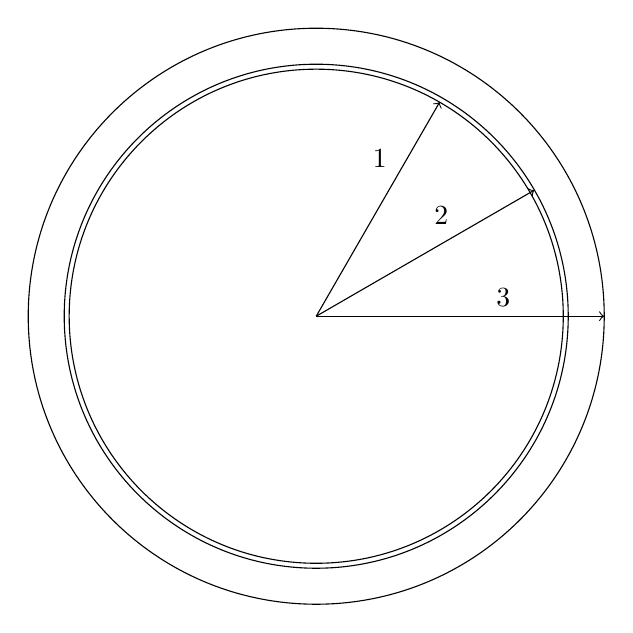
\begin{tikzpicture}[scale=8,auto]
        \draw (0,0) circle (0.39218);
      \draw[->] (0,0) -- node[pos=0.65] {1} (0.196,0.34);
      \draw (0,0) circle (0.40005);
      \draw[->] (0,0) -- node[pos=0.65] {2} (0.346,0.2);
      \draw (0,0) circle (0.4572);
      \draw[->] (0,0) -- node[pos=0.65] {3} (0.457,0.0);

      \end{tikzpicture}
      \begin{tikzpicture}
       \matrix [matrix of nodes]
      {
          Arrow & Radius (cm) & Material & \numrefheader \\
        1 & 0.39218 & \node[hyperlink node=mat_fuel16]{Fuel}; & \ref{num:fuelpellrad}\\ 
        2 & 0.40005 & \node[hyperlink node=mat_helium]{Helium}; & \ref{num:fuelIRrad}\\ 
        3 & 0.45720 & \node[hyperlink node=mat_zirc]{Zircaloy}; & \ref{num:fuelORrad}\\ 
      };
\end{tikzpicture}
\end{geoitem}
\begin{geoitem}{Upper Fuel Pin Plenum}{fig_fuel_pin_plenum}\centering
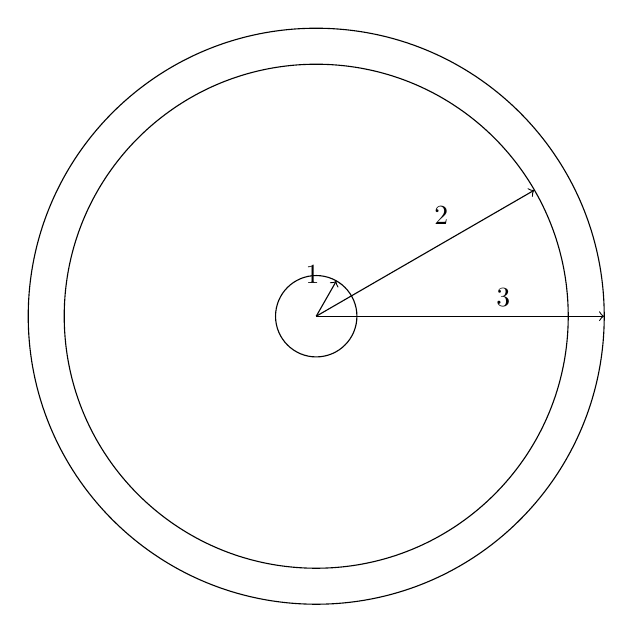
\begin{tikzpicture}[scale=8,auto]
        \draw (0,0) circle (0.06459);
      \draw[->] (0,0) -- node[pos=0.65] {1} (0.032,0.056);
      \draw (0,0) circle (0.40005);
      \draw[->] (0,0) -- node[pos=0.65] {2} (0.346,0.2);
      \draw (0,0) circle (0.4572);
      \draw[->] (0,0) -- node[pos=0.65] {3} (0.457,0.0);

      \end{tikzpicture}
      \begin{tikzpicture}
       \matrix [matrix of nodes]
      {
          Arrow & Radius (cm) & Material & \numrefheader \\
        1 & 0.06459 & \node[hyperlink node=mat_inconel]{Inconel}; & \ref{num:plenum_spring}\\ 
        2 & 0.40005 & \node[hyperlink node=mat_helium]{Helium}; & \ref{num:fuelIRrad}\\ 
        3 & 0.45720 & \node[hyperlink node=mat_zirc]{Zircaloy}; & \ref{num:fuelORrad}\\ 
      };
\end{tikzpicture}
\\ \raggedright This shows the radial geometry used in the upper
plenum region of the fuel pins, with a small mass of Inconel to approximate the
spring.
\end{geoitem}

\begin{geoitem}{Empty Guide Tube Geometry above Dashpot}{fig_guidetube_pin}\centering
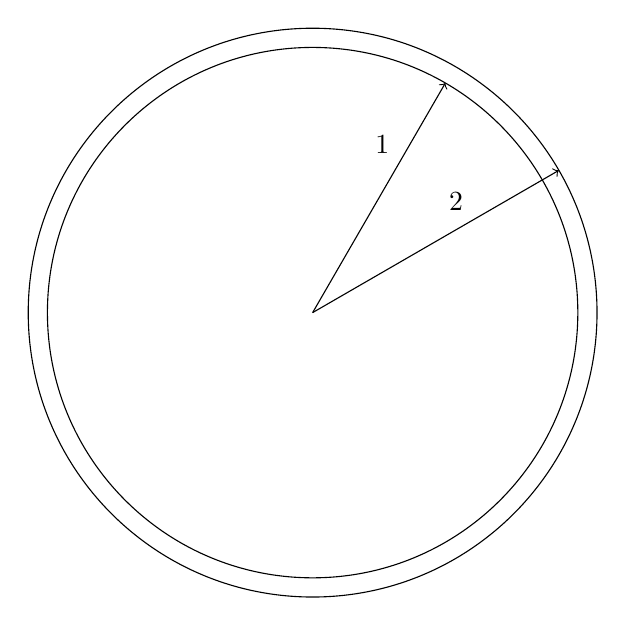
\begin{tikzpicture}[scale=6,auto]
        \draw (0,0) circle (0.56134);
      \draw[->] (0,0) -- node[pos=0.65] {1} (0.281,0.486);
      \draw (0,0) circle (0.60198);
      \draw[->] (0,0) -- node[pos=0.65] {2} (0.521,0.301);

      \end{tikzpicture}
      \begin{tikzpicture}
       \matrix [matrix of nodes]
      {
          Arrow & Radius (cm) & Material & \numrefheader \\
        1 & 0.56134 & \node[hyperlink node=mat_water]{Water}; & \ref{num:GTIRrad}\\ 
        2 & 0.60198 & \node[hyperlink node=mat_zirc]{Zircaloy}; & \ref{num:GTORrad}\\ 
      };
\end{tikzpicture}
\end{geoitem}
\begin{geoitem}{Empty Guide Tube Geometry at Dashpot}{fig_guidetube_da_pin}\centering
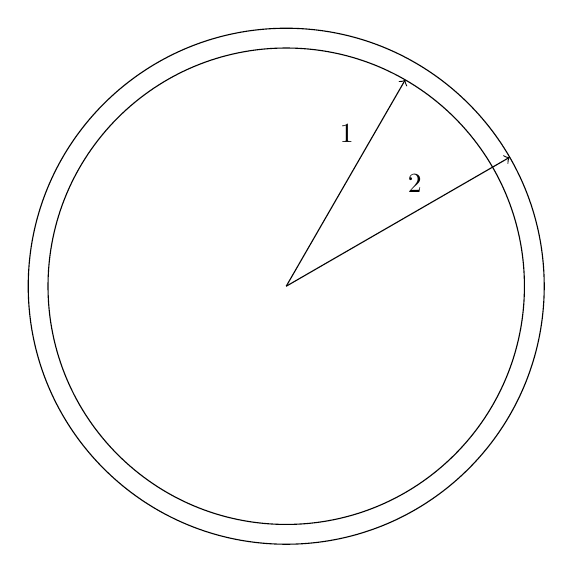
\begin{tikzpicture}[scale=6,auto]
        \draw (0,0) circle (0.50419);
      \draw[->] (0,0) -- node[pos=0.65] {1} (0.252,0.437);
      \draw (0,0) circle (0.5461);
      \draw[->] (0,0) -- node[pos=0.65] {2} (0.473,0.273);

      \end{tikzpicture}
      \begin{tikzpicture}
       \matrix [matrix of nodes]
      {
          Arrow & Radius (cm) & Material & \numrefheader \\
        1 & 0.50419 & \node[hyperlink node=mat_water]{Water}; & \ref{num:GTDPIRrad}\\ 
        2 & 0.54610 & \node[hyperlink node=mat_zirc]{Zircaloy}; & \ref{num:GTDPORrad}\\ 
      };
\end{tikzpicture}
\end{geoitem}

\begin{geoitem}{Instrument Tube Pin Geometry}{fig_instr_pin}\centering
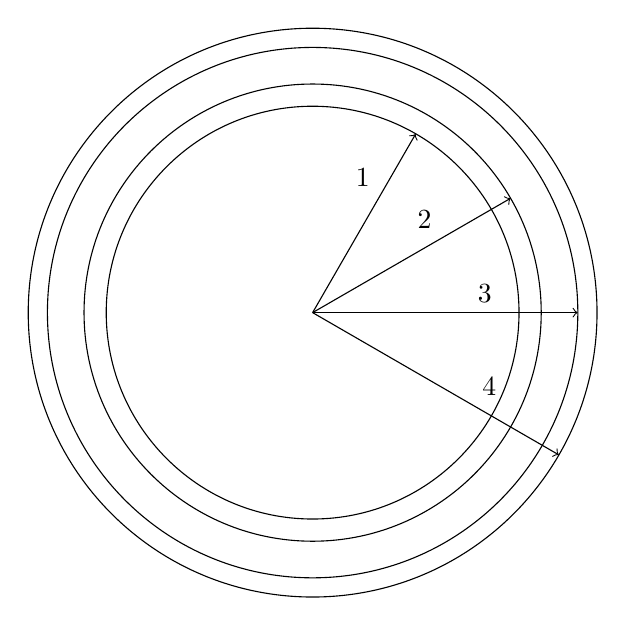
\begin{tikzpicture}[scale=6,auto]
        \draw (0,0) circle (0.43688);
      \draw[->] (0,0) -- node[pos=0.65] {1} (0.218,0.378);
      \draw (0,0) circle (0.48387);
      \draw[->] (0,0) -- node[pos=0.65] {2} (0.419,0.242);
      \draw (0,0) circle (0.56134);
      \draw[->] (0,0) -- node[pos=0.65] {3} (0.561,0.0);
      \draw (0,0) circle (0.60198);
      \draw[->] (0,0) -- node[pos=0.65] {4} (0.521,-0.301);

      \end{tikzpicture}
      \begin{tikzpicture}
       \matrix [matrix of nodes]
      {
          Arrow & Radius (cm) & Material & \numrefheader \\
        1 & 0.43688 & \node[hyperlink node=mat_air]{Air}; & \ref{num:ITthimIR}\\ 
        2 & 0.48387 & \node[hyperlink node=mat_zirc]{Zircaloy}; & \ref{num:ITthimOR}\\ 
        3 & 0.56134 & \node[hyperlink node=mat_water]{Water}; & \ref{num:GTIRrad}\\ 
        4 & 0.60198 & \node[hyperlink node=mat_zirc]{Zircaloy}; & \ref{num:GTORrad}\\ 
      };
\end{tikzpicture}
\\ \raggedright The thimble radii were chosen to be equivalent to the outer
thimble radii of control rods and burnable absorber rods by assumption. Note
that not all instrument tube positions contain the thimble defined by the first
2 radii in the diagram above, as discussed in Section \ref{sec:coreinstrpos}.
This pincell does not change at the dashpot.
\end{geoitem}

\begin{geoitem}{Bare Instrument Thimble Pin Geometry}{fig_instr_pin_bare}\centering
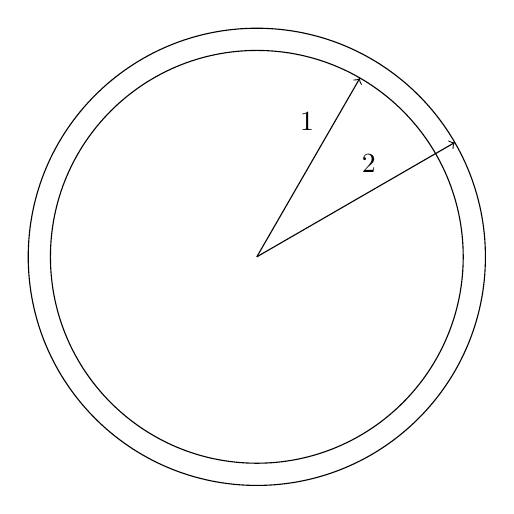
\begin{tikzpicture}[scale=6,auto]
        \draw (0,0) circle (0.43688);
      \draw[->] (0,0) -- node[pos=0.65] {1} (0.218,0.378);
      \draw (0,0) circle (0.48387);
      \draw[->] (0,0) -- node[pos=0.65] {2} (0.419,0.242);

      \end{tikzpicture}
      \begin{tikzpicture}
       \matrix [matrix of nodes]
      {
          Arrow & Radius (cm) & Material & \numrefheader \\
        1 & 0.43688 & \node[hyperlink node=mat_air]{Air}; & \ref{num:ITthimIR}\\ 
        2 & 0.48387 & \node[hyperlink node=mat_zirc]{Zircaloy}; & \ref{num:ITthimOR}\\ 
      };
\end{tikzpicture}
\\ \raggedright The bare instrument thimble for regions below the instrument tube.
\end{geoitem}

\begin{geoitem}{\acs{BP} Geometry above Dashpot}{fig_ba_pin}\centering
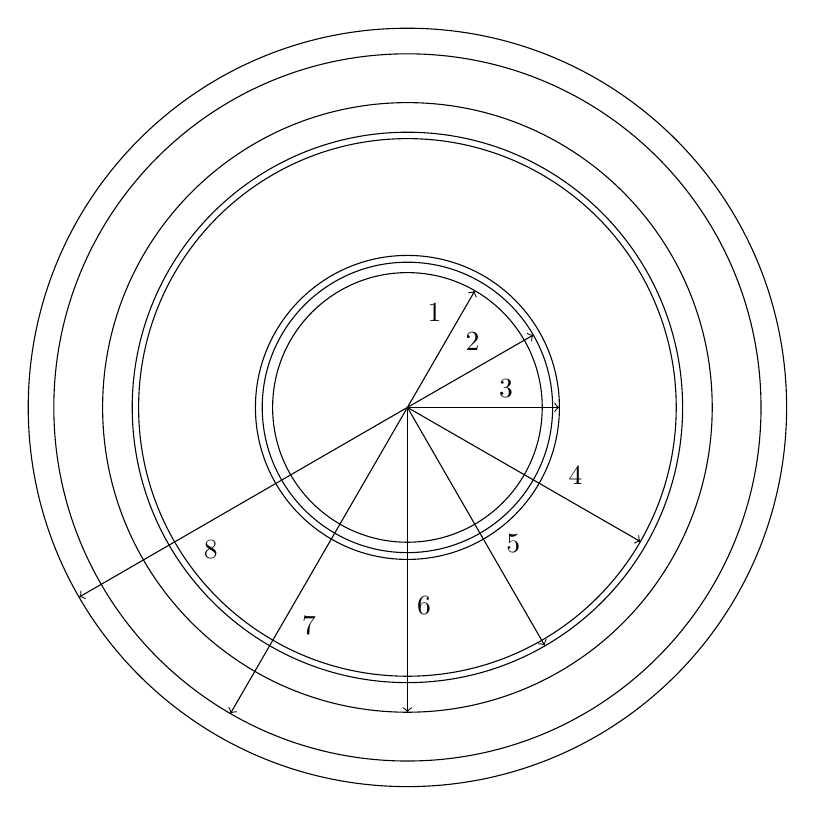
\begin{tikzpicture}[scale=8,auto]
        \draw (0,0) circle (0.214);
      \draw[->] (0,0) -- node[pos=0.65] {1} (0.107,0.185);
      \draw (0,0) circle (0.23051);
      \draw[->] (0,0) -- node[pos=0.65] {2} (0.2,0.115);
      \draw (0,0) circle (0.2413);
      \draw[->] (0,0) -- node[pos=0.65] {3} (0.241,0.0);
      \draw (0,0) circle (0.42672);
      \draw[->] (0,0) -- node[pos=0.65] {4} (0.37,-0.213);
      \draw (0,0) circle (0.43688);
      \draw[->] (0,0) -- node[pos=0.65] {5} (0.218,-0.378);
      \draw (0,0) circle (0.48387);
      \draw[->] (0,0) -- node[pos=0.65] {6} (0.0,-0.484);
      \draw (0,0) circle (0.56134);
      \draw[->] (0,0) -- node[pos=0.65] {7} (-0.281,-0.486);
      \draw (0,0) circle (0.60198);
      \draw[->] (0,0) -- node[pos=0.65] {8} (-0.521,-0.301);

      \end{tikzpicture}
      \begin{tikzpicture}
       \matrix [matrix of nodes]
      {
          Arrow & Radius (cm) & Material & \numrefheader \\
        1 & 0.21400 & \node[hyperlink node=mat_air]{Air}; & \ref{num:BPinnercladIR}\\ 
        2 & 0.23051 & \node[hyperlink node=mat_SS304]{SS304}; & \ref{num:BPinnercladOR}\\ 
        3 & 0.24130 & \node[hyperlink node=mat_helium]{Helium}; & \ref{num:BPpoisonIR}\\ 
        4 & 0.42672 & \node[hyperlink node=mat_borosilicate]{Borosilicate Glass}; & \ref{num:BPpoisonOR}\\ 
        5 & 0.43688 & \node[hyperlink node=mat_helium]{Helium}; & \ref{num:BPoutercladIR}\\ 
        6 & 0.48387 & \node[hyperlink node=mat_SS304]{SS304}; & \ref{num:BPoutercladOR}\\ 
        7 & 0.56134 & \node[hyperlink node=mat_water]{Water}; & \ref{num:GTIRrad}\\ 
        8 & 0.60198 & \node[hyperlink node=mat_zirc]{Zircaloy}; & \ref{num:GTORrad}\\ 
      };
\end{tikzpicture}
\end{geoitem}
\begin{geoitem}{\acs{BP} Plenum Geometry}{fig_ba_pin_plenum}\centering
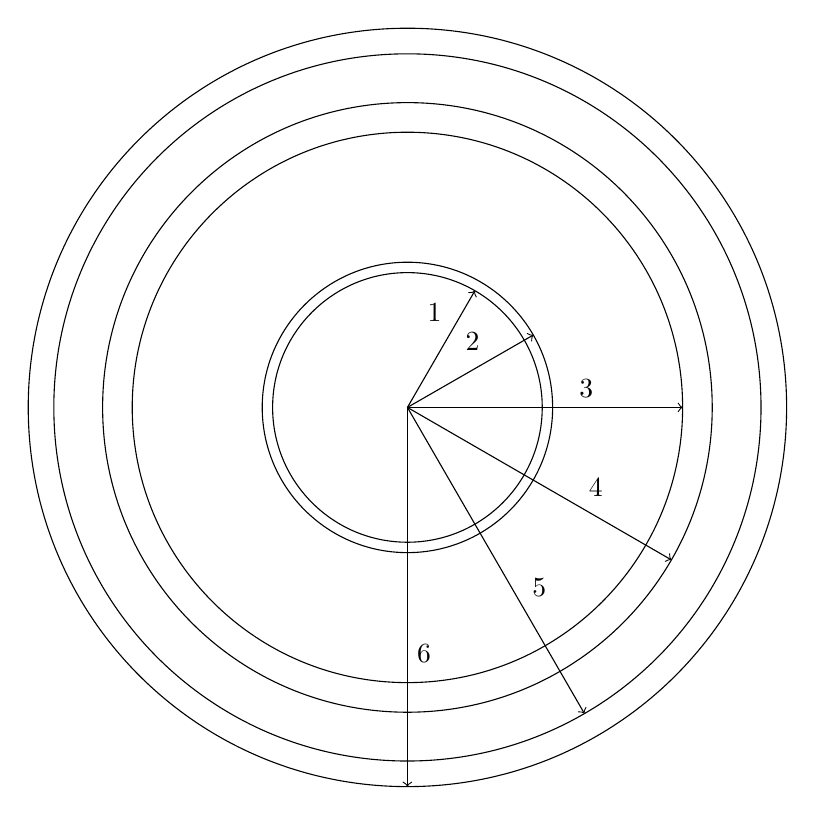
\begin{tikzpicture}[scale=8,auto]
        \draw (0,0) circle (0.214);
      \draw[->] (0,0) -- node[pos=0.65] {1} (0.107,0.185);
      \draw (0,0) circle (0.23051);
      \draw[->] (0,0) -- node[pos=0.65] {2} (0.2,0.115);
      \draw (0,0) circle (0.43688);
      \draw[->] (0,0) -- node[pos=0.65] {3} (0.437,0.0);
      \draw (0,0) circle (0.48387);
      \draw[->] (0,0) -- node[pos=0.65] {4} (0.419,-0.242);
      \draw (0,0) circle (0.56134);
      \draw[->] (0,0) -- node[pos=0.65] {5} (0.281,-0.486);
      \draw (0,0) circle (0.60198);
      \draw[->] (0,0) -- node[pos=0.65] {6} (0.0,-0.602);

      \end{tikzpicture}
      \begin{tikzpicture}
       \matrix [matrix of nodes]
      {
          Arrow & Radius (cm) & Material & \numrefheader \\
        1 & 0.21400 & \node[hyperlink node=mat_air]{Air}; & \ref{num:BPinnercladIR}\\ 
        2 & 0.23051 & \node[hyperlink node=mat_SS304]{SS304}; & \ref{num:BPinnercladOR}\\ 
        3 & 0.43688 & \node[hyperlink node=mat_helium]{Helium}; & \ref{num:BPoutercladIR}\\ 
        4 & 0.48387 & \node[hyperlink node=mat_SS304]{SS304}; & \ref{num:BPoutercladOR}\\ 
        5 & 0.56134 & \node[hyperlink node=mat_water]{Water}; & \ref{num:GTIRrad}\\ 
        6 & 0.60198 & \node[hyperlink node=mat_zirc]{Zircaloy}; & \ref{num:GTORrad}\\ 
      };
\end{tikzpicture}
\end{geoitem}

\begin{figure}[htbp]
    \centering
    \begin{tikzpicture}[scale=1,x=1in,y=1in]
      \node[inner sep=0pt,
        text width=3.4 in,
        minimum size=0.222222222222 in,
        draw=black,
        align=center,
        shift={(0,0.0)},
        hyperlink node=mat_water] (n0) {Water};
      \draw[->] (1.9,-0.111111111111) node[right,anchor=west] {0.00000 ~~~~~~~ Lowest Extent} -- (1.7,-0.111111111111);
      \node[anchor=east] (s0) at (n0.west) {};
      \node[inner sep=0pt,
        text width=3.4 in,
        minimum size=0.222222222222 in,
        draw=black,
        align=center,
        shift={(0,0.222222222222)},
        hyperlink node=mat_water_spn] (n1) {Support Plate / Nozzle Borated Water};
      \draw[->] (1.9,0.111111111111) node[right,anchor=west] {20.0000 ~~~~~~~ Bottom of Support Plate} -- (1.7,0.111111111111);
      \node[anchor=east] (s1) at (n1.west) {\ref{num:missing}};
      \node[inner sep=0pt,
        text width=3.4 in,
        minimum size=0.222222222222 in,
        draw=black,
        align=center,
        shift={(0,0.444444444444)},
        hyperlink node=mat_water] (n2) {Water};
      \draw[->] (1.9,0.333333333333) node[right,anchor=west] {35.0000 ~~~~~~~ Bottom of Fuel Rod} -- (1.7,0.333333333333);
      \node[anchor=east] (s2) at (n2.west) {};
      \node[inner sep=0pt,
        text width=3.4 in,
        minimum size=0.222222222222 in,
        draw=black,
        align=center,
        shift={(0,0.666666666667)},
        hyperlink node=mat_SS304] (n3) {Stainless Steel Pin};
      \draw[->] (1.9,0.555555555556) node[right,anchor=west] {39.9580 ~~~~~~~ Bottom of Control Rod} -- (1.7,0.555555555556);
      \node[anchor=east] (s3) at (n3.west) {\ref{num:control_rod_axials}};
      \node[inner sep=0pt,
        text width=3.4 in,
        minimum size=0.222222222222 in,
        draw=black,
        align=center,
        shift={(0,0.888888888889)},
        hyperlink node=fig_cr_pin] (n4) {Control Rod Lower Absorber Pincell};
      \draw[->] (1.9,0.777777777778) node[right,anchor=west] {41.8280 ~~~~~~~ Bottom of Lower Absorber (AIC)} -- (1.7,0.777777777778);
      \node[anchor=east] (s4) at (n4.west) {\ref{num:control_rod_axials}};
      \node[inner sep=0pt,
        text width=3.4 in,
        minimum size=0.222222222222 in,
        draw=black,
        align=center,
        shift={(0,1.11111111111)},
        hyperlink node=fig_cr_pin_upper] (n5) {Control Rod Upper Absorber Pincell};
      \draw[->] (1.9,1.0) node[right,anchor=west] {143.428 ~~~~~~~ Bottom of Upper Absorber (B4C)} -- (1.7,1.0);
      \node[anchor=east] (s5) at (n5.west) {\ref{num:control_rod_axials}};
      \node[inner sep=0pt,
        text width=3.4 in,
        minimum size=0.222222222222 in,
        draw=black,
        align=center,
        shift={(0,1.33333333333)},
        hyperlink node=fig_cr_pin_spacer] (n6) {Control Rod Spacer Pincell};
      \draw[->] (1.9,1.22222222222) node[right,anchor=west] {402.508 ~~~~~~~ Bottom of Spacer} -- (1.7,1.22222222222);
      \node[anchor=east] (s6) at (n6.west) {\ref{num:control_rod_axials}};
      \node[inner sep=0pt,
        text width=3.4 in,
        minimum size=0.222222222222 in,
        draw=black,
        align=center,
        shift={(0,1.55555555556)},
        hyperlink node=fig_cr_pin_plenum] (n7) {Control Rod Upper Plenum};
      \draw[->] (1.9,1.44444444444) node[right,anchor=west] {403.778 ~~~~~~~ Bottom of Control Rod Plenum} -- (1.7,1.44444444444);
      \node[anchor=east] (s7) at (n7.west) {\ref{num:control_rod_axials}};
      \node[inner sep=0pt,
        text width=3.4 in,
        minimum size=0.222222222222 in,
        draw=black,
        align=center,
        shift={(0,1.77777777778)},
        hyperlink node=mat_SS304] (n8) {Stainless Steel Pin};
      \draw[->] (1.9,1.66666666667) node[right,anchor=west] {415.558 ~~~~~~~ Top of Control Rod Plenum} -- (1.7,1.66666666667);
      \node[anchor=east] (s8) at (n8.west) {\ref{num:control_rod_axials}};
      \path let \p1 = (n8.west) in node[anchor=west] (source) at (\x1,2.11111111111) {\underline{Source Reference}};
      \draw[->] (source.west) -| (s8.north);
      \draw[->] (1.9,1.88888888889) node[right,anchor=west] {460.000 ~~~~~~~ Highest Extent} -- (1.7,1.88888888889);
      \draw (1.7,2.11111111111) node[right,anchor=west] {\underline{Elevation (cm)} ~ \underline{Description}};

    \end{tikzpicture}


    \caption[Control rod pincell axial specification]{Control rod pincell axial specification when fully-inserted.  This only shows axial sections for the control rod itself, which is inside one of the guide tubes.\label{fig_cr_axials}}
\end{figure}
